\apendice{Documentación de usuario}

\section{Requisitos software y hardware para ejecutar el proyecto}

Para ejecutar este proyecto, se requieren los siguientes componentes de software y hardware:

\subsection{Software}
El desarrollo de la página web en streamlit, requiere unos requisitos específicos de software clave para que todo funcione correctamente.

\subsubsection{Descripción de los elementos software necesarios y sus respectivas funciones}
\begin{itemize}
\item \textbf{Python}: Lenguaje de programación principal para desarrollar los scripts que manejan la adquisición y análisis de datos \cite{Python}.
\item \textbf{Streamlit}: Herramienta para crear la interfaz web que permite la visualización de datos en tiempo real y la interacción con el usuario \cite{Streamlit}.
\item \textbf{Tkinter}: Utilizado para crear la ventana de escritorio que muestra los datos en vivo y permite grabarlos \cite{Tkinter}.
\item \textbf{Tkinter}: PowerShell de Anaconda: Terminal utilizada para ejecutar scripts y notebooks de análisis de datos \cite{PowerShell}.
\item \textbf{Jupyter Notebook}: Utilizado para el desarrollo y la documentación del proceso de tratamiento de datos y la elección del modelo de predicción \cite{Jupyter}.
\item \textbf{Arduino IDE}: Necesario para programar y cargar el script en la placa Arduino \cite{ArduinoLanguage}.
\item \textbf{Librerías de Python}: Varias librerías son necesarias para el correcto funcionamiento de los scripts, incluyendo:
\begin{itemize}
\item \textbf{pyserial}: Para la comunicación serial entre el Arduino y el ordenador.
\item \textbf{pandas}: Para el manejo y análisis de datos.
\item \textbf{numpy}: Para operaciones matemáticas y de matriz.
\item \textbf{scikit-learn}: Para la implementación del modelo de machine learning.
\item \textbf{matplotlib}: Para la visualización de datos y gráficos.
\end{itemize}
\end{itemize}

\subsubsection{Requisitos de software}
Los requisitos de software aseguran el correcto funcionamiento del prototipo de monitorización del ECG. Su descripción esta en las tablas RF-01 (Tabla \ref{RF-01}) a RF-06 (Tabla \ref{RF-06}).

\begin{table}[p]
    \centering
    \begin{tabularx}{\linewidth}{ p{0.21\columnwidth} p{0.71\columnwidth} }
        \toprule
        \textbf{RF-01}    & \textbf{Aplicación web}\\
        \toprule
        \textbf{Descripción}              & El proyecto debe contar con una interfaz web que permita la visualización en tiempo real del ECG, la grabación de estos datos en formato CSV, y su posterior análisis.   \\
        \textbf{Importancia}                & Alta, ya que proporciona la interfaz principal para la interacción del usuario con el sistema. \\
        \textbf{Prioridad}                & Alta, fundamental para el acceso y manejo de los datos de ECG. \\
        \bottomrule
    \end{tabularx}
    \caption{RF-01 Aplicación web}
    \label{RF-01}
\end{table}

\begin{table}[p]
    \centering
    \begin{tabularx}{\linewidth}{ p{0.21\columnwidth} p{0.71\columnwidth} }
        \toprule
        \textbf{RF-02}    & \textbf{Recolección y grabación de datos}\\
        \toprule
        \textbf{Descripción}              & La solución debe permitir la visualización en tiempo real de los datos de ECG y ofrecer la opción de grabar estos datos en un archivo .xls.   \\
        \textbf{Importancia}                & Alta, porque facilita la captura y revisión posterior de los datos. \\
        \textbf{Prioridad}                & Alta, esencial para la funcionalidad de registro de datos. \\
        \bottomrule
    \end{tabularx}
    \caption{RF-02 Recolección y grabación de datos}
    \label{RF-02}
\end{table}

\begin{table}[p]
    \centering
    \begin{tabularx}{\linewidth}{ p{0.21\columnwidth} p{0.71\columnwidth} }
        \toprule
        \textbf{RF-03}    & \textbf{Análisis y Predicción de Datos}\\
        \toprule
        \textbf{Descripción}              & El sistema debe proporcionar una funcionalidad para cargar datos de ECG desde un archivo, segmentar estos datos en ciclos cardíacos, y predecir el tipo de cada ciclo.   \\
        \textbf{Importancia}                & Alta, crucial para el análisis detallado y diagnóstico basado en ECG. \\
        \textbf{Prioridad}                & Alta, proporciona el valor clínico central del sistema. \\
        \bottomrule
    \end{tabularx}
    \caption{RF-03 Análisis y predicción de datos}
    \label{RF-03}
\end{table}

\begin{table}[p]
    \centering
    \begin{tabularx}{\linewidth}{ p{0.21\columnwidth} p{0.71\columnwidth} }
        \toprule
        \textbf{RF-04}    & \textbf{Visualización de resultados de análisis}\\
        \toprule
        \textbf{Descripción}              & La interfaz debe ofrecer una representación visual clara de los resultados del análisis, incluyendo la clasificación de los ciclos cardíacos y cualquier dato relevante.   \\
        \textbf{Importancia}                & Alta, esencial para la interpretación inmediata y efectiva de los resultados por parte del usuario. \\
        \textbf{Prioridad}                & Alta, impacta directamente en la utilidad clínica del sistema. \\
        \bottomrule
    \end{tabularx}
    \caption{RF-04 Visualización de resultados de análisis}
    \label{RF-04}
\end{table}

\begin{table}[p]
    \centering
    \begin{tabularx}{\linewidth}{ p{0.21\columnwidth} p{0.71\columnwidth} }
        \toprule
        \textbf{RF-05}    & \textbf{Gestión de base de datos}\\
        \toprule
        \textbf{Descripción}              & Debe permitirse almacenar y gestionar las predicciones de los tipos de ciclo cardíaco en una base de datos, junto con la fecha y hora de cada registro, y ofrecer la posibilidad de eliminar las filas por si ocurre un error.   \\
        \textbf{Importancia}                & Media, facilita el almacenamiento a largo plazo y la revisión de los datos. \\
        \textbf{Prioridad}                & Media, complementa la funcionalidad de análisis del sistema. \\
        \bottomrule
    \end{tabularx}
    \caption{RF-05 Gestión de base de datos}
    \label{RF-05}
\end{table}

\begin{table}[p]
    \centering
    \begin{tabularx}{\linewidth}{ p{0.21\columnwidth} p{0.71\columnwidth} }
        \toprule
        \textbf{RF-06}    & \textbf{Descarga de datos}\\
        \toprule
        \textbf{Descripción}              & Proporcionar una funcionalidad que permita a los usuarios descargar las predicciones en formatos estándares que puedan ser utilizados para consultas médicas o almacenamiento personal.   \\
        \textbf{Importancia}                & Media, proporciona flexibilidad y portabilidad de los datos. \\
        \textbf{Prioridad}                & Media, mejora la interoperabilidad y la integración con otros sistemas. \\
        \bottomrule
    \end{tabularx}
    \caption{RF-06 Descarga de datos}
    \label{RF-06}
\end{table}


\subsection{Hardware}
Para que el proyecto funcione correctamente, es necesario tener el hardware adecuado que se complemente con el software desarrollado. Se han realizado ajustes y adiciones al hardware del prototipo original para hacerlo más fácil de usar y cómodo. La Tabla \ref{tabla-costes-hardware} muestra todos los componentes utilizados.


\begin{table}[]
    \centering
    \begin{tabular}{|c|c|}
    \hline
    \rowcolor[HTML]{FFFFFF} 
    \multicolumn{2}{|c|}{\cellcolor[HTML]{FFFFFF}\textbf{Componentes}} \\ \hline 
    \rowcolor[HTML]{EFEFEF} 
    Arduino UNO R3 & Electrodos \\ \hline
    \rowcolor[HTML]{FFFFFF} 
    Cables & Módulo AD8232 \\ \hline
    \rowcolor[HTML]{EFEFEF} 
    Caja 3D & LED \\ \hline
    \rowcolor[HTML]{FFFFFF} 
    Resistencias & \\ \hline
    \end{tabular}
    \caption{Componentes del prototipo de monitorización de ECG.}
    \label{tabla-componentes-hardware}
\end{table}

\subsubsection{Requisitos de Hardware}
Los requisitos de hardware aseguran el correcto funcionamiento del prototipo de monitorización del ECG. Su descripción esta en las tablas RF-07 (Tabla \ref{RF-07}) a RF-09 (Tabla \ref{RF-09}).

\begin{table}[p]
    \centering
    \begin{tabularx}{\linewidth}{ p{0.21\columnwidth} p{0.71\columnwidth} }
        \toprule
        \textbf{RF-07}    & \textbf{Transmisión de datos por USB} \\
        \toprule
        \textbf{Descripción}              & El dispositivo debe ser capaz de transmitir los datos del sensor AD8232 al ordenador mediante una conexión USB, garantizando una comunicación estable y rápida.   \\
        \textbf{Importancia}                & Alta \\
        \textbf{Prioridad}                & Alta \\
        \bottomrule
    \end{tabularx}
    \caption{RF-07 Transmisión de datos por USB}
    \label{RF-07}
\end{table}

\begin{table}[p]
    \centering
    \begin{tabularx}{\linewidth}{ p{0.21\columnwidth} p{0.71\columnwidth} }
        \toprule
        \textbf{RF-8}    & \textbf{Alimentación a través de USB} \\
        \toprule
        \textbf{Descripción}              & El prototipo debe poder alimentarse directamente desde el puerto USB del ordenador, eliminando la necesidad de una fuente de alimentación externa.   \\
        \textbf{Importancia}                & Alta \\
        \textbf{Prioridad}                & Alta \\
        \bottomrule
    \end{tabularx}
    \caption{RF-8 Alimentación a través de USB}
    \label{RF-8}
\end{table}


\begin{table}[p]
    \centering
    \begin{tabularx}{\linewidth}{ p{0.21\columnwidth} p{0.71\columnwidth} }
        \toprule
        \textbf{RF-9}    & \textbf{Seguridad y manejabilidad del prototipo} \\
        \toprule
        \textbf{Descripción}              & Es crucial que todos los componentes del hardware estén bien protegidos y asegurados dentro de la caja de protección impresa en 3D. Esto no solo garantiza la seguridad del usuario, sino también la durabilidad del dispositivo.   \\
        \textbf{Importancia}                & Alta \\
        \textbf{Prioridad}                & Alta \\
        \bottomrule
    \end{tabularx}
    \caption{RF-9 Seguridad y manejabilidad del prototipo}
    \label{RF-09}
\end{table}


\section{Instalación y puesta en marcha}

Se ha escrito una guía para que los usuarios puedan instalar y utilizar el proyecto de manera efectiva, siguiendo los pasos necesarios para preparar el dispositivo y desplegar la aplicación web que hay a continuación.

Antes de comenzar, hay que instalar y configurar los siguientes programas: Anaconda Navigator y Arduino IDE.

\subsection{Configuración del dispositivo}
\begin{enumerate}
    \item \textbf{Carga del Programa en Arduino}:
    \begin{itemize}
        \item 1. Conecte la placa Arduino al ordenador mediante un cable USB.
        \item 2. Abra el Arduino IDE y cargue el archivo \textit{Arduino/version 2/AD82\_usb\_y\_led.ino}.
        \item 3. Compila y sube el programa a la placa Arduino (Ver Figura \ref{fig:arduino}).
        \item 4. Mantenga la placa Arduino conectada al ordenador a través del cable USB.
    \end{itemize}
\end{enumerate}

\begin{figure}[h]
    \centering
    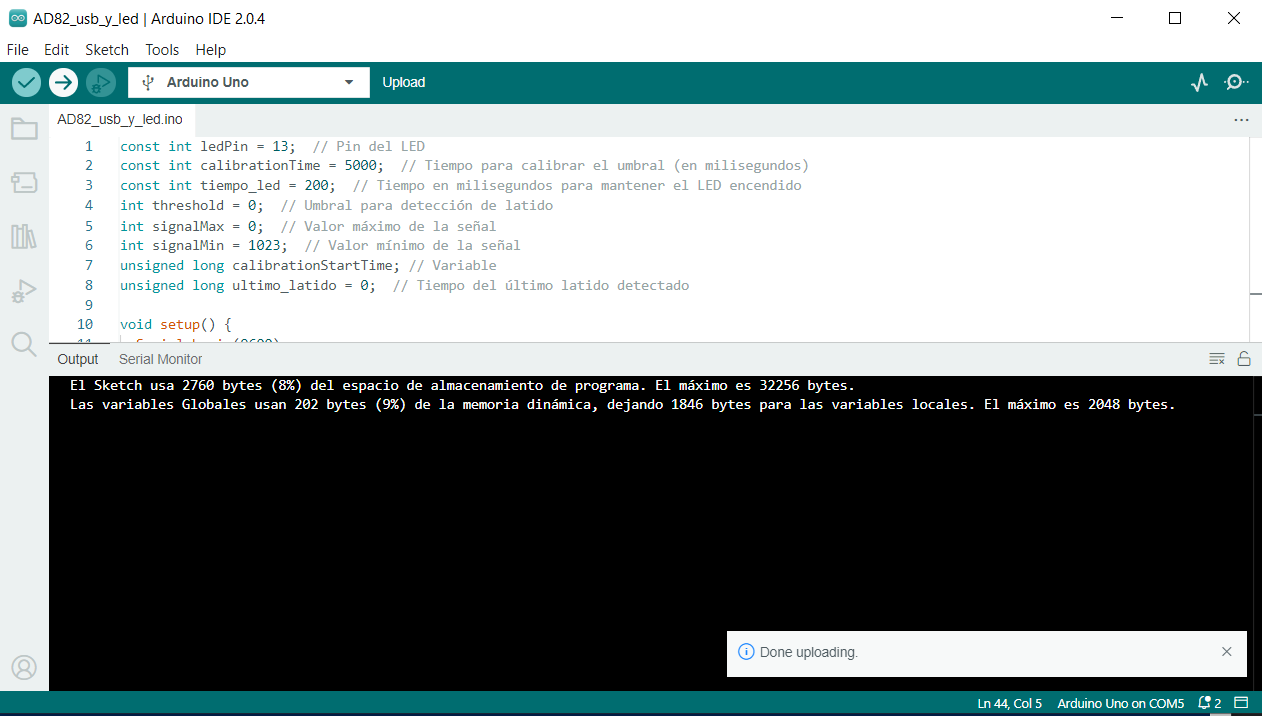
\includegraphics[width=0.8\textwidth]{img/arduino.png}
    \caption{Carga del programa en la placa Arduino.}
    \label{fig:arduino}
\end{figure}

\subsection{Abrir la aplicación web en entorno local}

\subsubsection{Instalación de Librerías Necesarias}
\begin{itemize}
    \item En la terminal de Anaconda, asegúrate de tener instaladas las siguientes librerías de Python:
     \begin{itemize}
            \item \textbf{streamlit}: \texttt{pip install streamlit}
            \item \textbf{pandas}: \texttt{pip install pandas}
            \item \textbf{numpy}: \texttt{pip install numpy}
            \item \textbf{matplotlib}: \texttt{pip install matplotlib}
            \item \textbf{scipy}: \texttt{pip install scipy}
            \item \textbf{joblib}: \texttt{pip install joblib}
            \item \textbf{pillow}: \texttt{pip install pillow}
        \end{itemize}
\end{itemize}

\subsubsection{Preparación del entorno con Anaconda Navigator}
\begin{enumerate}
    \item Abre Anaconda Navigator en su ordenador.
    \item Accede a la terminal (CMD.exe Prompt) desde Anaconda Navigator.
    \item Navega hasta el directorio del proyecto utilizando el comando \texttt{cd TFG} (Ver Figura \ref{fig:ejecutar}).
    \item Asegúrese de tener todos los archivos necesarios en la carpeta, incluyendo \textit{streamlit.py}, \textit{serialmonitor.py} y el modelo de predicción ya entrenado (\textit{ecg\_model.pkl}).
\end{enumerate}

\begin{figure}[h]
    \centering
    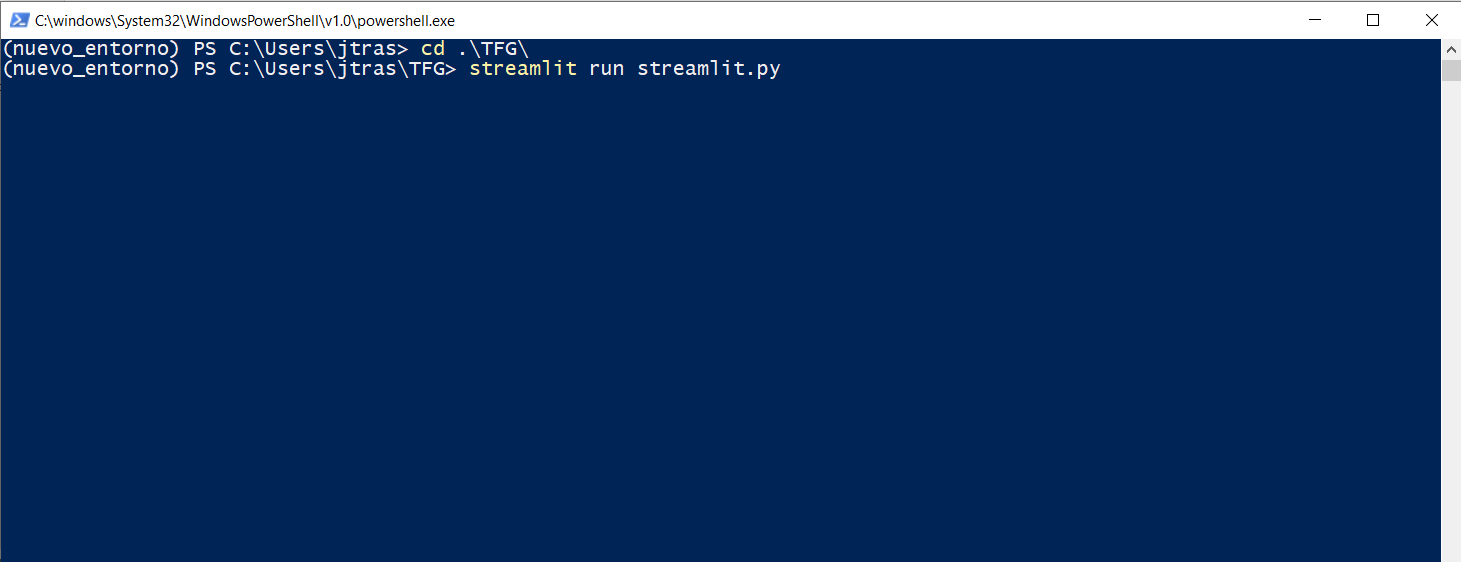
\includegraphics[width=0.8\textwidth]{img/cd.png}
    \caption{Navegación al directorio del proyecto en la terminal de Anaconda.}
    \label{fig:ejecutar}
\end{figure}

\subsubsection{Ejecución de la aplicación web}
\begin{enumerate}
    \item En la terminal de Anaconda, ejecute el comando \texttt{streamlit run streamlit.py} (Ver Figura \ref{fig:ejecutar2}).
    \item Si el proceso es exitoso, se abrirá una nueva ventana en su navegador web mostrando la interfaz de la aplicación.
\end{enumerate}

\begin{figure}[h]
    \centering
    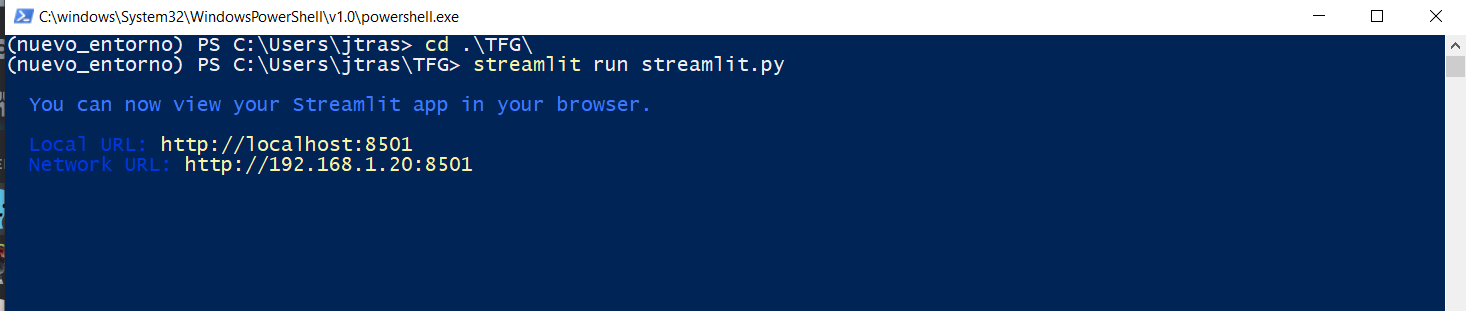
\includegraphics[width=0.8\textwidth]{img/cd2.png}
    \caption{Ejecución de la aplicación web con Streamlit.}
    \label{fig:ejecutar2}
\end{figure}


\subsection{Interacción con la aplicación}
\begin{enumerate}
    \item \textbf{Visualización de Datos en Tiempo Real}:
    \begin{itemize}
        \item Con la aplicación web abierta, la pantalla Datos en Vivo te permitirá visualizar los datos de ECG en tiempo real.
        \item Asegúrate de que el Arduino esté correctamente conectado y enviando datos al ordenador.
    \end{itemize}

    \item \textbf{Grabación de datos}:
    \begin{itemize}
        \item Desde la ventana de escritorio, selecciona la opción para iniciar la grabación de datos de ECG.
        \item Los datos grabados se almacenarán en un archivo Excel para su posterior análisis.
    \end{itemize}

    \item \textbf{Análisis de datos}:
    \begin{itemize}
        \item En la aplicación web, navega hasta la sección de análisis de datos.
        \item Sube el archivo Excel con los datos de ECG grabados.
        \item El modelo de predicción analizará los datos y generará etiquetas para cada ciclo cardíaco.
    \end{itemize}

    \item \textbf{Gestión de la base de datos}:
    \begin{itemize}
        \item Las predicciones generadas se pueden almacenar en la base de datos junto con la fecha y hora de la grabación.
        \item También puedes descargar la base de datos en formato CSV para realizar análisis adicionales o consultar a un profesional de salud.
    \end{itemize}
\end{enumerate}



\section{Manuales y/o Demostraciones prácticas}

\subsection{Manuales}

\subsubsection{Preparación}
Esta sección proporciona instrucciones claras para que cualquier persona pueda usar el producto, incluso si nunca lo ha utilizado antes.

\begin{enumerate}
    \item \textbf{Colocar y encender el dispositivo}:
    \begin{itemize}
        \item Coloca correctamente los electrodos del sensor AD8232 en el cuerpo, tal y como se indica en la foto \ref{fig:electrodosreal}. Estate seguro de que estén bien sujetos.
        \item Realice todos los pasos de la instalación hasta conseguir tener abierta la aplicación web en el navegador que se esta utilizando antes de pasar al siguiente paso.
    \end{itemize}
\end{enumerate}

\subsubsection{Utilización}
La página web ofrece distintas funcionalidades para los usuarios que se explicaran brevemente a continuación y de forma mas detallada en el vídeo demostrativo subido al \href{https://github.com/diegotrascasa/TFG_Diego_Trascasa_Garcia}{repositorio de GitHub}.

\begin{itemize}
    \item \textbf{Visualización de datos en tiempo real}:
    \begin{itemize}
        \item En la ventana de la web datos en vivo abierta, hay que pulsar el botón de abrir ventana de monitoreo cardiaco \ref{fig:tkinter}, donde tras seleccionar el puerto COM correcto y abrir el serial se podrá visualizar los datos de ECG en tiempo real.
    \end{itemize}

    \item \textbf{Grabación de datos }:
    \begin{itemize}
        \item Desde la ventana de monitoreo cardiaco \ref{fig:tkinter}, seleccione la opción para iniciar la grabación de datos de ECG.
        \item Los datos grabados se almacenarán en un archivo Excel para su posterior análisis.
    \end{itemize}

    \item \textbf{Análisis de datos}:
    \begin{itemize}
        \item En la aplicación web, navega hasta la sección de análisis de datos, sube el archivo Excel con los datos de ECG grabados (ajusta, si es necesario la longitud de la grabación) y el modelo de predicción analizará los datos y generará etiquetas para cada ciclo cardíaco.
    \end{itemize}

    \item \textbf{Gestión de la base de datos}:
    \begin{itemize}
        \item Las predicciones generadas se pueden almacenar en la base de datos, junto con la fecha y hora de la grabación \ref{fig:database_management}. También cuenta con un botón para eliminar el id seleccionado en caso de que haya habido un error y además, se puede descargar la base de datos en formato .CSV para realizar estadísticas adicionales o consultar a un profesional de salud.
    \end{itemize}
\end{itemize}

\begin{figure}[h]
    \centering
    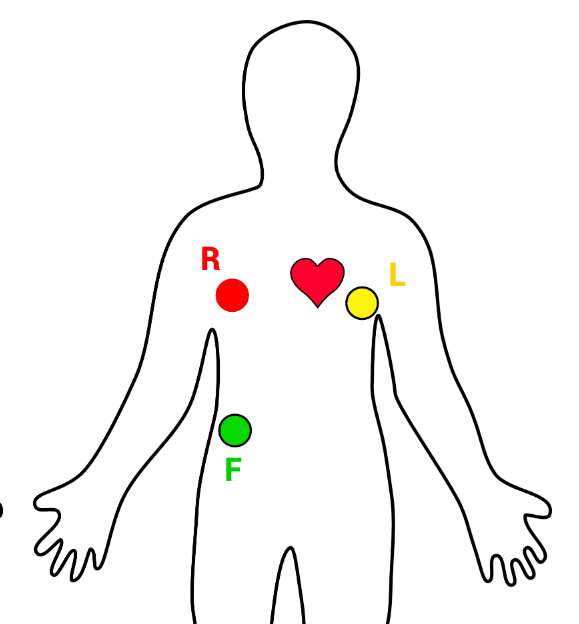
\includegraphics[width=0.8\textwidth]{img/electrodosreal.png}
    \caption{Colocación correcta de los electrodos del sensor AD8232 \cite{electrodos}.}
    \label{fig:electrodosreal}
\end{figure}


\begin{figure}[h]
    \centering
    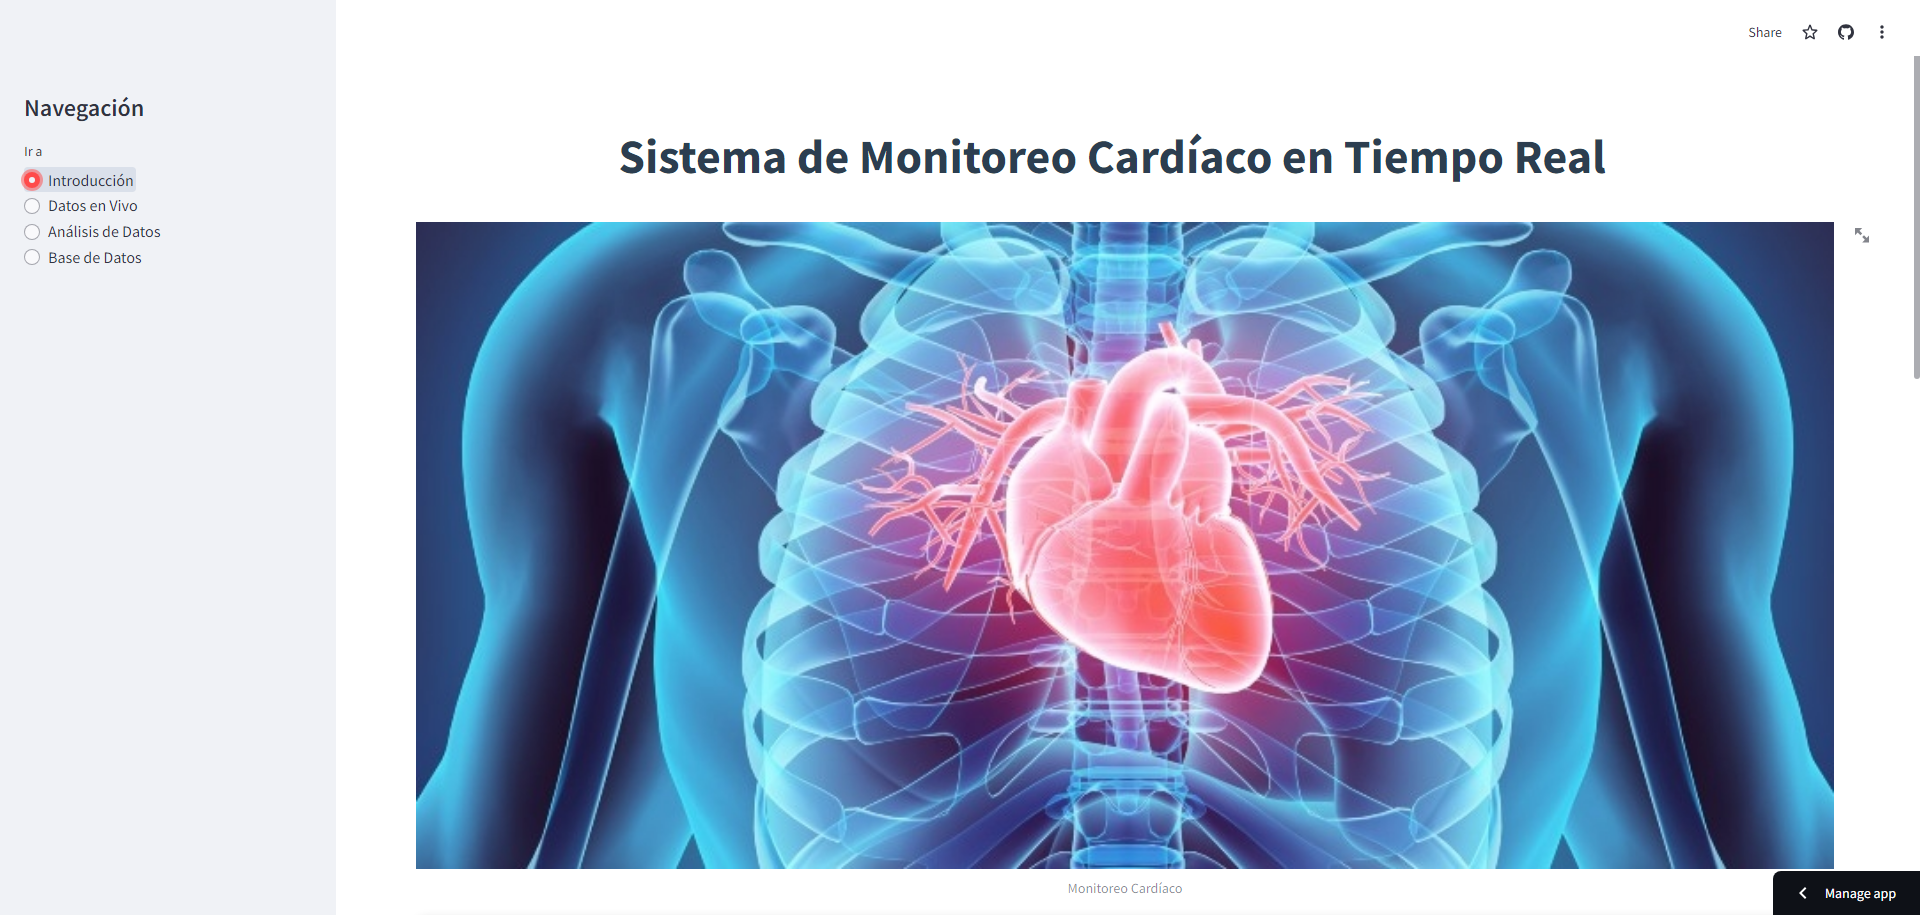
\includegraphics[width=0.8\textwidth]{img/interfaz_streamlit.png}
    \caption{Pantalla principal de la aplicación web desarrollada con Streamlit.}
    \label{fig:streamlit_main}
\end{figure}

\begin{figure}[h]
    \centering
    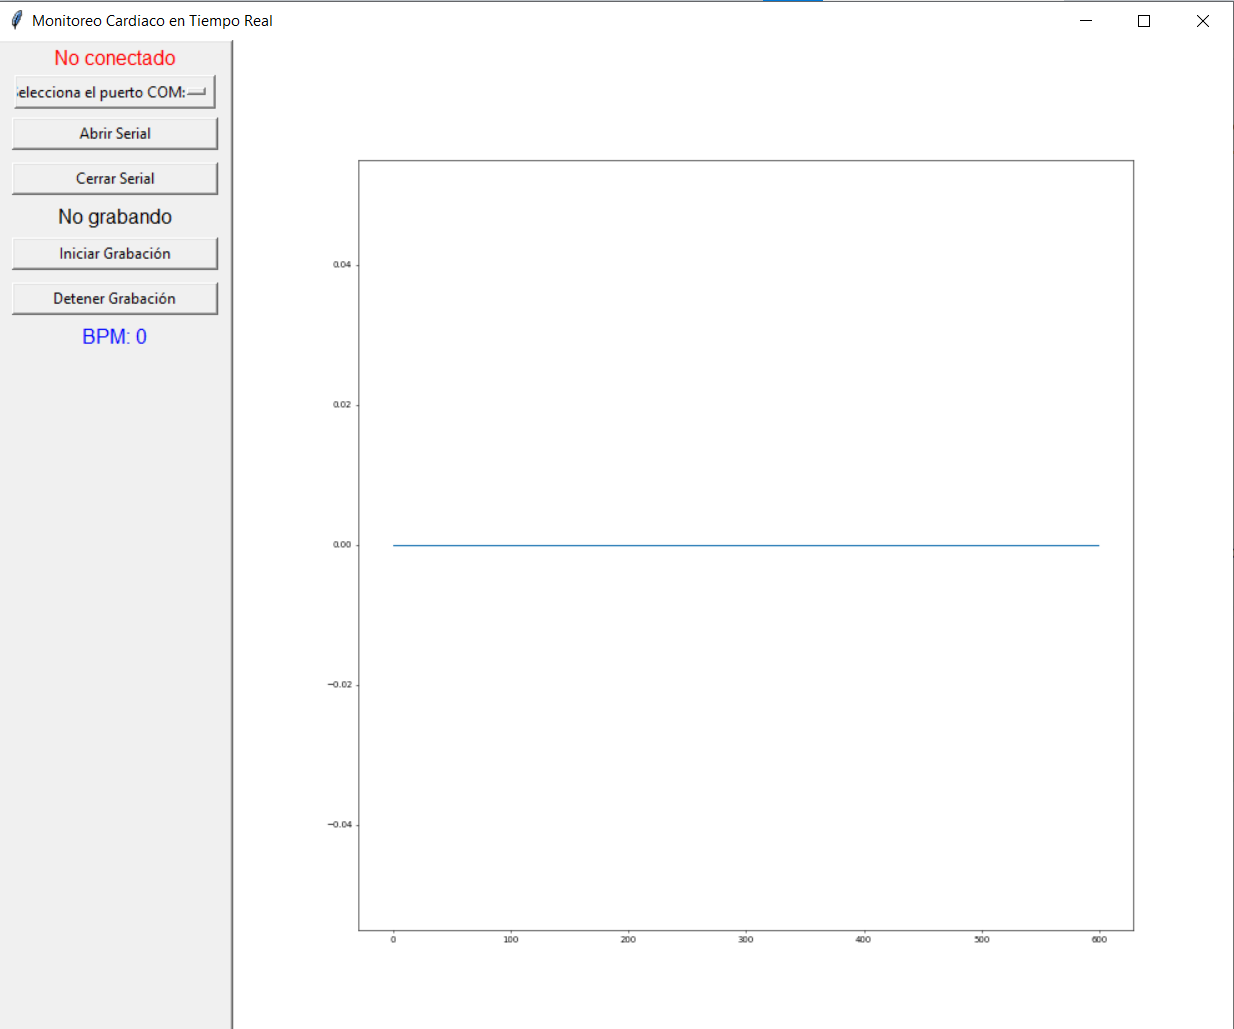
\includegraphics[width=0.8\textwidth]{img/ventana_tinker.png}
    \caption{Ventana de grabación de datos ECG en la aplicación web.}
    \label{fig:tkinter}
\end{figure}

\begin{figure}[h]
    \centering
    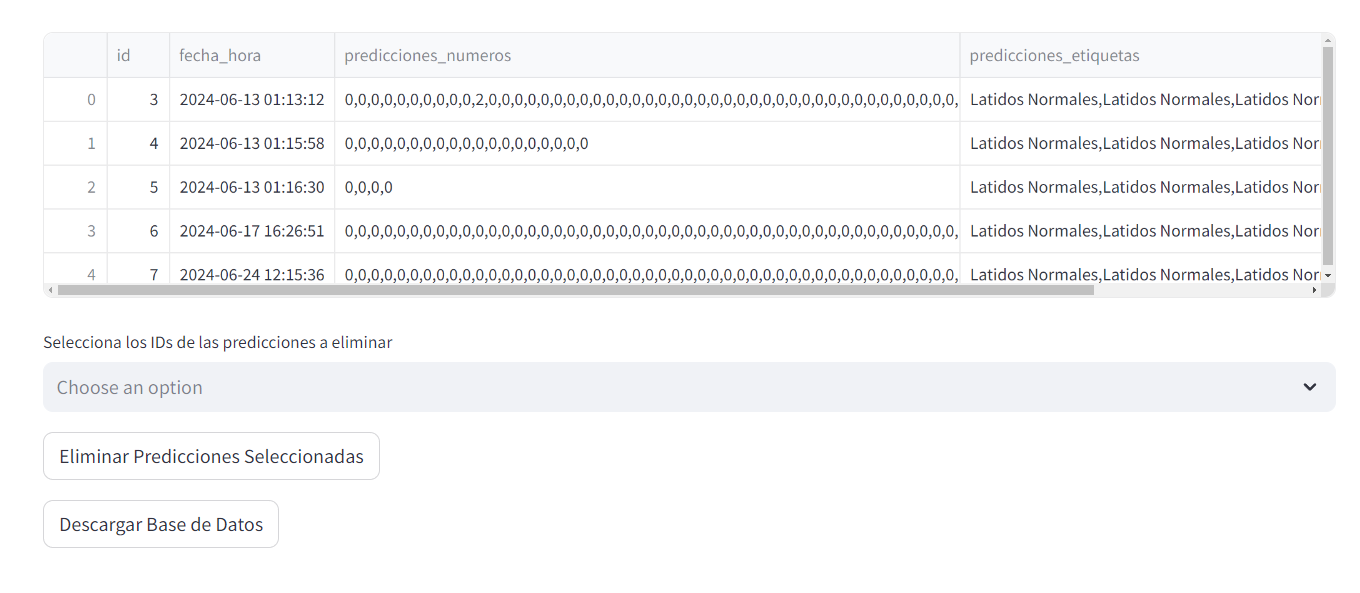
\includegraphics[width=0.8\textwidth]{img/bbdd.png}
    \caption{Gestión de la base de datos en la aplicación web.}
    \label{fig:database_management}
\end{figure}

\subsection{Demostraciones prácticas}

Para entender mejor tanto el proceso de instalación para que todo funcione correcto como las diferentes funcionalidades de la aplicación web se ha realizado un vídeo que esta subido en el respositorio GitHub con una demostración del funcionamiento completo del proyecto en \href{https://github.com/diegotrascasa/TFG}{repositorio de GitHub}

\begin{itemize}
    \item \textbf{Demostraciones}:
    \begin{itemize}
        \item Vídeo tutorial sobre cómo instalar y configurar el entorno de desarrollo.
        \item Ejemplos prácticos de cómo realizar la grabación de datos inicial con el dispositivo de monitoreo.
        \item Demostración en vídeo de las principales funcionalidades de la interfaz web.
        \item Ejemplos de análisis de diferentes datos.
    \end{itemize}
    
\end{itemize}